%%%%%%%%%%%%%%%%%%%%%%%%%%%%%%%%%%%%%%%%%%%%%%%%%%%%%%%%%%%%%%%%%%%%%
%
% CSCI 1430 Written Question Template
%
% This is a LaTeX document. LaTeX is a markup language for producing documents. 
% You will fill out this document, compile it into a PDF document, then upload the PDF to Gradescope. 
%
% To compile into a PDF on department machines:
% > pdflatex thisfile.tex
%
% If you do not have LaTeX, your options are:
% - VSCode extension: https://marketplace.visualstudio.com/items?itemName=James-Yu.latex-workshop
% - Online Tool: https://www.overleaf.com/ - most LaTeX packages are pre-installed here (e.g., \usepackage{}).
% - Personal laptops (all common OS): http://www.latex-project.org/get/ 
%
% If you need help with LaTeX, please come to office hours.
% Or, there is plenty of help online:
% https://en.wikibooks.org/wiki/LaTeX
%
% Good luck!
% Srinath and the 1430 staff
%
%%%%%%%%%%%%%%%%%%%%%%%%%%%%%%%%%%%%%%%%%%%%%%%%%%%%%%%%%%%%%%%%%%%%%

\documentclass[11pt]{article}

\usepackage[english]{babel}
\usepackage[utf8]{inputenc}
\usepackage{amssymb}
\usepackage{xcolor}
\usepackage[colorlinks = true,
            linkcolor = blue,
            urlcolor  = blue]{hyperref}
\usepackage[a4paper,margin=1.5in]{geometry}
\usepackage{stackengine,graphicx}
\usepackage{fancyhdr}
\setlength{\headheight}{15pt}
\usepackage{microtype}
\usepackage{times}
\usepackage[shortlabels]{enumitem}
\setlist[enumerate]{topsep=0pt}
\usepackage{amsmath}
\usepackage{framed}
\usepackage{mdframed}
\usepackage{xcolor}
\usepackage[most]{tcolorbox}

% a great python code format: https://github.com/olivierverdier/python-latex-highlighting
\usepackage{pythonhighlight}

\usepackage{trimclip,lipsum}

\frenchspacing
\setlength{\parindent}{0cm} % Default is 15pt.
\setlength{\parskip}{0.3cm plus1mm minus1mm}

\pagestyle{fancy}
\fancyhf{}
\lhead{Homework 2 Written Questions}
\rhead{CSCI 1430}
\lfoot{\textcolor{red}{\textbf{Only}
\ifcase\thepage
\or \textbf{instructions}
\or \textbf{Q1}
\or \textbf{A1}
\or \textbf{Q2}
\or \textbf{A2 (a)}
\or \textbf{A2 (b)}
\or \textbf{A2 (c)}
\or \textbf{A2 (d)}
\or \textbf{A3 (a) - (b)}
\or \textbf{A3 (c)}
\or \textbf{A4 (a)}
\or \textbf{A4 (b)}
\or \textbf{Q5}
\or \textbf{A5}
\or \textbf{A6}
\or \textbf{A6}
\or \textbf{discussion attendance}
\or \textbf{feedback}
\else
[ERROR: PAGE MISALIGNMENT]
\fi
\textbf{should be on this page}
}}
\rfoot{\thepage~/ 18}


\date{}

\title{\vspace{-1cm}Homework 2 Written Questions}


\begin{document}
\maketitle
\vspace{-3cm}
\thispagestyle{fancy}


\section*{ Document Instructions}
\begin{itemize}
  \item 6 questions \textbf{[3 + 11 + 9 + 6 + 3 + 3 = 35 points]}.
  \item Fill all your answers within the answer boxes, and \textbf{please do NOT remove the answer box outlines}.
  \item Questions are highlighted in the \textbf{orange boxes}, bonus questions are highlighted in \textbf{blue boxes}, answers should be recorded in the \textbf{green boxes}.
  \item Include code, images, and equations where appropriate.
  \item To identify all places where your responses are expected, search for `TODO'.
  \item The answer box sizes have been set by the staff beforehand and will truncate your text if it goes beyond the limit. Please make sure your responses fit in the appropriate spaces. \textbf{Extra pages are not permitted unless otherwise specified.}
  \item Make sure your submission has the right number of pages to validate page alignment sanity (check the footer).
  \item Please make this document anonymous.
\end{itemize}

\section*{ Gradescope Instructions}
\begin{itemize}
  \item When you are finished, compile this document to a PDF and submit it directly to Gradescope. 
  \item The pages will be automatically assigned to the right questions on Gradescope \textit{assuming you do not add any unnecessary pages}. \textbf{Inconsistently assigned pages will lead to a deduction of 2 points per misaligned page (capped at a maximum 6 point deduction).}
\end{itemize}
\pagebreak


\paragraph{Q1:} \textbf{[3 points]} Let's look again at the webcam Fourier decomposition demo which Srinath showed in class. 

The Fourier transform (or fast Fourier transform more specifically) is often regarded as one of the most important algorithms ever developed. The internet, your WiFi, smartphone, phone, computer, router, satellites, almost everything that has a computer inside uses these algorithms in one way or another to function. Below is a depiction of FFT being used for aircraft vibration analysis.

\begin{center}
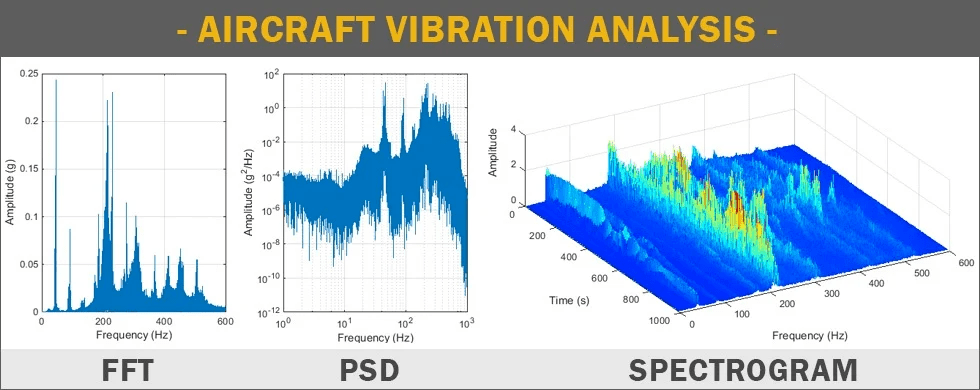
\includegraphics[width=300px,height=95px]{images/aircraft-vibration-analysis-plots.png} 
\end{center}

\begin{tcolorbox}[colback=orange!5!white,colframe=orange!75!black]
Navigate to the \texttt{questions} folder. Then, within your cs1430 virtual environment, run the following command:
\begin{verbatim}
$ python liveFFT2.py
\end{verbatim}

\textit{Warning: If you're running the code from within WSL, this will likely not work since you need access to your laptop's camera / webcam.}

This file contains five parts for you to explore and see the amplitude image, the phase image, and the effect of the reconstructed image.
\begin{itemize}
    \item Part 0: Scanning the basis and observing the output image.
    \item Part 1: Reconstructions from different numbers of basis frequencies.
    \item Part 2: Replacing amplitude and phase with that from a different image.
    \item Part 3: Replacing amplitude and phase with that from a noise image.
    \item Part 4: Manipulating the amplitude and phase images.
\end{itemize}

Uncomment the different parts and explore the camera feed decomposition! Please include three results of your experimentation. We'll be grading for completion, not correctness.

\emph{Note:} For anonymous grading, try not to put yourself in the camera frame. Show your favourite vector calculus book, wear a mask, use your cat, etc. Extra credit for creative effort.
\end{tcolorbox}

\begin{tcolorbox}[colback=white!5!white,colframe=green!75!black]

\includegraphics[width=1\textwidth,height=7cm,keepaspectratio]{images/TODO wall-e.jpg}

\includegraphics[width=1\textwidth,height=7cm,keepaspectratio]{images/TODO wall-e.jpg}

\includegraphics[width=1\textwidth,height=7cm,keepaspectratio]{images/TODO wall-e.jpg}
\end{tcolorbox}

%%%%%%%%%%%%%%%%%%%%%%%%%%%%%%%%%%%

% % Please leave the pagebreak
% \pagebreak
% \section*{Exercise Results}
% Please include images of your results from the exercise here, e.g., two-to-three screenshots of your findings.



% \pagebreak
% Extra space


%%%%%%%%%%%%%%%%%%%%%%%%%%%%%%%%%%%


%%%%%%%%%%%%%%%%%%%%%%%%%%%%%%%%%%%

% Please leave the pagebreak
\pagebreak

\paragraph{Q2:} \textbf{[11 points]} Imagine you wished to find points in one image which matched to the same world point in another image. This is called feature point correspondence matching.

In direct feature matching, correspondences are established with simple and fast nearest neighbor searches between multidimensional embeddings. Closest points reveal in fact the best compromise between intensity and spatial location.

\begin{center}
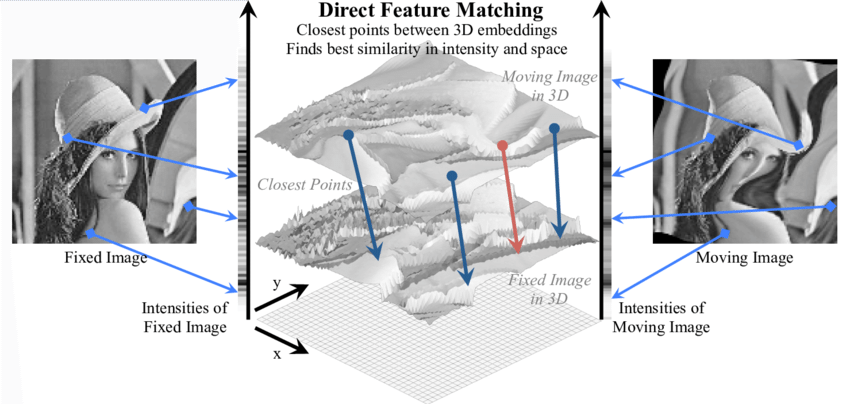
\includegraphics[width=300px,height=125px]{images/Direct-Feature-Matching-Correspondences-are-established-with-simple-and-fast-nearest.png} 
\end{center}

\begin{tcolorbox}[colback=orange!5!white,colframe=orange!75!black]
Please use the included python script \texttt{plot\_corners.py} to find corners using Harris corner detection for each pair of images below. 

For each pair, discuss the differences in the returned corners (if any), the aspects of the images that create these differences, and any underlying real world phenomena that may have been the primary cause of these differences. \textbf{[3-5 sentences]}
\end{tcolorbox}

\pagebreak
\begin{enumerate}[(a)]
    \item \textbf{[1 + 2 points]}
RISHLibrary: 
\href{images/RISHLibrary1.jpg}{RISHLibrary1.jpg} and \href{images/RISHLibrary2.jpg}{RISHLibrary2.jpg} 
\begin{tcolorbox}[colback=white!5!white,colframe=green!75!black,breakable]
%%%%%%% ANSWER STARTS HERE %%%%%%%%%%%%%%%%%%%%%%%%%%%%
%%%%%%% Replace TODO wall-e.jpg with your picture %%%%%

\includegraphics[width=1\textwidth,height=7cm,keepaspectratio]{images/TODO wall-e.jpg}

\includegraphics[width=1\textwidth,height=7cm,keepaspectratio]{images/TODO wall-e.jpg}

\setbox0=\hbox{\parbox[t]{\textwidth}{

TODO: Your answer for (a) here

%%%%%%% ANSWER ENDS HERE %%%%%%%%%%%%%%%%%%%%%%%%%%%%%%
}}
\clipbox{0pt \dimexpr\dp0-7\baselineskip\relax{} 0in 0pt}{\copy0}
\end{tcolorbox}

\pagebreak
\item \textbf{[1 + 2 points]}
Chase:
\href{images/Chase1.jpg}{Chase1.jpg} and \href{images/Chase2.jpg}{Chase2.jpg}
\begin{tcolorbox}[colback=white!5!white,colframe=green!75!black]
%%%%%%% ANSWER STARTS HERE %%%%%%%%%%%%%%%%%%%%%%%%%%%%
%%%%%%% Replace TODO wall-e.jpg with your picture %%%%%

\includegraphics[width=1\textwidth,height=7cm,keepaspectratio]{images/TODO wall-e.jpg}

\includegraphics[width=1\textwidth,height=7cm,keepaspectratio]{images/TODO wall-e.jpg}

\setbox0=\hbox{\parbox[t]{\textwidth}{

TODO: Your answer for (b) here

%%%%%%% ANSWER ENDS HERE %%%%%%%%%%%%%%%%%%%%%%%%%%%%%%
}}
\clipbox{0pt \dimexpr\dp0-7\baselineskip\relax{} 0in 0pt}{\copy0}
\end{tcolorbox}

\pagebreak
\item \textbf{[1 + 2 points]} 
LaddObservatory: 
\href{images/LaddObservatory1.jpg}{LaddObservatory1.jpg} and \href{images/LaddObservatory2.jpg}{LaddObservatory2.jpg}
\begin{tcolorbox}[colback=white!5!white,colframe=green!75!black]

%%%%%%% ANSWER STARTS HERE %%%%%%%%%%%%%%%%%%%%%%%%%%%%
%%%%%%% Replace TODO wall-e.jpg with your picture %%%%%

\includegraphics[width=1\textwidth,height=7cm,keepaspectratio]{images/TODO wall-e.jpg}

\includegraphics[width=1\textwidth,height=7cm,keepaspectratio]{images/TODO wall-e.jpg}

\setbox0=\hbox{\parbox[t]{\textwidth}{

TODO: Your answer for (c) here

%%%%%%% ANSWER ENDS HERE %%%%%%%%%%%%%%%%%%%%%%%%%%%%%%
}}
\clipbox{0pt \dimexpr\dp0-6\baselineskip\relax{} 0in 0pt}{\copy0}
\end{tcolorbox}

\pagebreak
\item \textbf{[2 points]} In the coding portion of the homework, you'll investigate strategies to filter only the matches you are most confident in. What problems could be caused if someone took feature matching algorithm results to be 100\% accurate? \textbf{[3-4 sentences]}

\begin{tcolorbox}[colback=white!5!white,colframe=green!75!black]
\setbox0=\hbox{\parbox[t]{\textwidth}{
    %%%%%%% ANSWER STARTS HERE %%%%%%%%%%%%%%%%%%%%%%%%%%%%
        
    TODO: Your answer for (d) here
        
    %%%%%%% ANSWER ENDS HERE %%%%%%%%%%%%%%%%%%%%%%%%%%%%%%
    }}
\clipbox{0pt \dimexpr\dp0-6\baselineskip\relax{} 0in 0pt}{\copy0}
\end{tcolorbox}
\end{enumerate}

\pagebreak
\paragraph{Q3:} \textbf{[9 points]} One use of local feature extraction and matching is \href{https://www.youtube.com/watch?v=xD88Qs_DZp4}{fingerprint recognition}---please watch the video and note the similarity to our task in this homework. Fingerprint recognition uses biometric data---measurements of human biological features that are unique to an individual---to make it convenient to unlock doors or devices quickly and without needing to remember a password. However, given its uniqueness, biometric data may be seen as a greater privacy encroachment upon a person than a password. Further, given the trust that is derived from the uniqueness of biometric data, it may also pose a greater risk of misuse if the data is not secure because the data cannot be changed.

\begin{enumerate}[(a)]
    \item \textbf{[2 + 1 points]}
    \begin{tcolorbox}[colback=orange!5!white,colframe=orange!75!black]
    Do you use biometric recognition systems? List them. [If not, list some that people around you use.]
    For one of the systems you use, where is the reference data stored (such as your stored fingerprint), and where and how does the authentication process happen (at a high level)? 
    Try to find the answer online; \href{https://ievoreader.com/how-biometric-data-is-stored/}{this article} may also help. \textbf{[4-6 sentences]}
    \end{tcolorbox}
    
    \begin{tcolorbox}[colback=white!5!white,colframe=green!75!black]
    \setbox0=\hbox{\parbox[t]{\textwidth}{
        %%%%%%% ANSWER STARTS HERE %%%%%%%%%%%%%%%%%%%%%%%%%%%%
            
        TODO: Your answer for (a) here
            
        %%%%%%% ANSWER ENDS HERE %%%%%%%%%%%%%%%%%%%%%%%%%%%%%%
        }}
    \clipbox{0pt \dimexpr\dp0-9\baselineskip\relax{} 0in 0pt}{\copy0}
    \end{tcolorbox}

    \item
    \textbf{[3 points]}
    \begin{tcolorbox}[colback=orange!5!white,colframe=orange!75!black]
    How might someone use computer vision to steal or spoof your biometric data to gain access? \emph{This could be across reconstruction, recognition, or (re)organization.} \textbf{[3-5 sentences]}
    \end{tcolorbox}

    \begin{tcolorbox}[colback=white!5!white,colframe=green!75!black]
    \setbox0=\hbox{\parbox[t]{\textwidth}{
        %%%%%%% ANSWER STARTS HERE %%%%%%%%%%%%%%%%%%%%%%%%%%%%
            
        TODO: Your answer for (b) here
            
        %%%%%%% ANSWER ENDS HERE %%%%%%%%%%%%%%%%%%%%%%%%%%%%%%
        }}
    \clipbox{0pt \dimexpr\dp0-8\baselineskip\relax{} 0in 0pt}{\copy0}
    \end{tcolorbox}


    \pagebreak
    \item
    \textbf{[3 points]}
    \begin{tcolorbox}[colback=orange!5!white,colframe=orange!75!black]
    Biometric recognition systems may not affect all people equally. For a biometric authentication system, define a group of people and describe how they might be affected disproportionately. \textbf{[3-5 sentences]}
    \end{tcolorbox}
    
    \begin{tcolorbox}[colback=white!5!white,colframe=green!75!black]
    \setbox0=\hbox{\parbox[t]{\textwidth}{
        %%%%%%% ANSWER STARTS HERE %%%%%%%%%%%%%%%%%%%%%%%%%%%%
            
        TODO: Your answer for (c) here
            
        %%%%%%% ANSWER ENDS HERE %%%%%%%%%%%%%%%%%%%%%%%%%%%%%%
        }}
    \clipbox{0pt \dimexpr\dp0-8\baselineskip\relax{} 0in 0pt}{\copy0}
    \end{tcolorbox}
\end{enumerate}

\pagebreak


%%%%%%%%%%%%%%%%%%%%%%%%%%%%%%%%%%%

\paragraph{Q4:} \textbf{[6 points]} Brown University decides to entirely replace passwords with biometric data to authenticate student identity on its computer systems. Given how accurate your feature matching homework 2 code is, Brown asks you to develop the authentication system as your CSCI 1430 final project. Lucky you.

As preparation, you read a previous case about a \href{https://www.vpnmentor.com/blog/report-biostar2-leak/}{biometric data breach}.

\begin{enumerate}[(a)]
    \item \textbf{[1 + 2 points]}
    \begin{tcolorbox}[colback=orange!5!white,colframe=orange!75!black]
    How were BioStar 2 storing their fingerprint data? Knowing the computer vision algorithms involved in feature matching, what different processing, features, or storage might you consider instead to decrease the risk of a biometric data breach? \textbf{[4-6 sentences]}
    \end{tcolorbox}

    \begin{tcolorbox}[colback=white!5!white,colframe=green!75!black]
    \setbox0=\hbox{\parbox[t]{\textwidth}{
        %%%%%%% ANSWER STARTS HERE %%%%%%%%%%%%%%%%%%%%%%%%%%%%
            
        TODO: Your answer for (a) here
            
        %%%%%%% ANSWER ENDS HERE %%%%%%%%%%%%%%%%%%%%%%%%%%%%%%
        }}
    \clipbox{0pt \dimexpr\dp0-8\baselineskip\relax{} 0in 0pt}{\copy0}
    \end{tcolorbox}

    \pagebreak
    \item 
    \textbf{[2 + 1 points]}
Even though fingerprints are thought to be unique, we are bound by the accuracy of computer vision systems to detect and recognize that uniqueness.
This may be a challenge for Brown's 10,000 students, let alone a national-scale database such as the FBI's \href{https://www.fbi.gov/services/cjis/fingerprints-and-other-biometrics/ngi}{Next Generation Identification System} that houses over 100 million fingerprints; its Advanced Fingerprint Identification Technology is claimed to be 99.6\% accurate.

Even seemingly high accuracies can create many inaccurate matches with large databases, potentially causing inaccurage judgements in criminal cases. 

    \begin{tcolorbox}[colback=orange!5!white,colframe=orange!75!black]
    Compare the causes that affect matching performance in natural images in Q2 to those that you might expect within the scenario of fingerprint recognition for door or device unlocking. Based on this, is accurate fingerprint recognition an easier problem than natural image matching? \textbf{[5-7 sentences]}

    \emph{Refer to the video at the beginning of Q3 and \href{http://biometrics.cse.msu.edu/Presentations/AnilJain_UniquenessOfFingerprints_NAS05.pdf}{this slide deck} for example images and additional information.}
    \end{tcolorbox}

    \begin{tcolorbox}[colback=white!5!white,colframe=green!75!black]
    \setbox0=\hbox{\parbox[t]{\textwidth}{
        %%%%%%% ANSWER STARTS HERE %%%%%%%%%%%%%%%%%%%%%%%%%%%%
            
        TODO: Your answer for (b) here
            
        %%%%%%% ANSWER ENDS HERE %%%%%%%%%%%%%%%%%%%%%%%%%%%%%%
        }}
    \clipbox{0pt \dimexpr\dp0-10\baselineskip\relax{} 0in 0pt}{\copy0}
    \end{tcolorbox}

\end{enumerate}

\pagebreak


%%%%%%%%%%%%%%%%%%%%%%%%%%%%%%%%%%%

% Please leave the pagebreak

\pagebreak
\paragraph{Q5:} \textbf{[3 points]}
Consider the pictures below of the same mountain.

\begin{center}
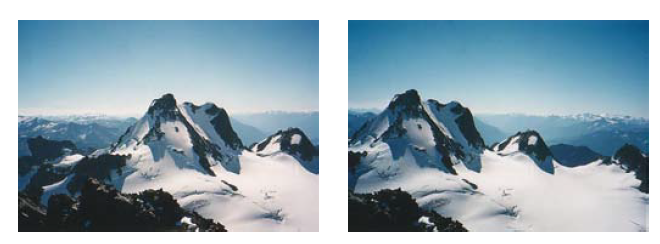
\includegraphics[width=300px,height=125px]{images/harris_mountains.png} 
\end{center}

If you were tasked with the problem of stitching them together to form a panoramic view, what would be the first thing you would think of doing?  You would probably find points in one image which appear in the other.

The Harris Corner Detector is commonly used in computer vision algorithms to find interest points from which to extract stable features for image matching.

To detect these features, we attempt to determine the strength of any change in the Energy (intensity) function $E(u, v)$ on the image. Since we can approximate corner points to be represented by quadratic-esque energy level surfaces, we can use the Taylor expansion and quantify the change in $E(u, v)$ within a certain radius in the image.

You might remember from your Calculus class that the second partial derivative test helps us determine if a point is a local min, local max or saddle point. Similarly, we focus on the second derivative term in the Taylor expansion to determine the shape of $E(u, v)$ and determine if that particular point is a corner or not.

Now, we can represent the Taylor expansion using matrices, and so the second derivative can be expressed as a matrix. Specifically, this matrix, $M$, is called the second moment matrix.

\textit{Note:} For a more comprehensive background, review the lecture slides.

\begin{tcolorbox}[colback=orange!5!white,colframe=orange!75!black]
How do the eigenvalues of the `M' second moment matrix vary with local image brightness, and how might we interpret the eigenvalues geometrically (think `shape')? \textbf{6-8 sentences}
\end{tcolorbox}

\begin{tcolorbox}[colback=white!5!white,colframe=green!75!black]
\setbox0=\hbox{\parbox[t]{\textwidth}{
    %%%%%%% ANSWER STARTS HERE %%%%%%%%%%%%%%%%%%%%%%%%%%%%
        
    TODO: Your answer for Q5 here
        
    %%%%%%% ANSWER ENDS HERE %%%%%%%%%%%%%%%%%%%%%%%%%%%%%%
    }}
\clipbox{0pt \dimexpr\dp0-14\baselineskip\relax{} 0in 0pt}{\copy0}
\end{tcolorbox}

% Please leave the pagebreak
\pagebreak
\paragraph{Q6:} \textbf{[3 points]}
Once you've detected the feature points, the next step is to extract their descriptions, i.e., their general properties. These generated feature descriptors will be used in the final step when matching feature points via their feature descriptors.

The algorithm to use here to extract the feature descriptors of feature points is SIFT. Given a interest point location, the SIFT algorithm converts a 16$\times$16 patch around the interest point into a 128$\times$1 feature descriptor of the gradient magnitudes and orientations therein.

\begin{center}
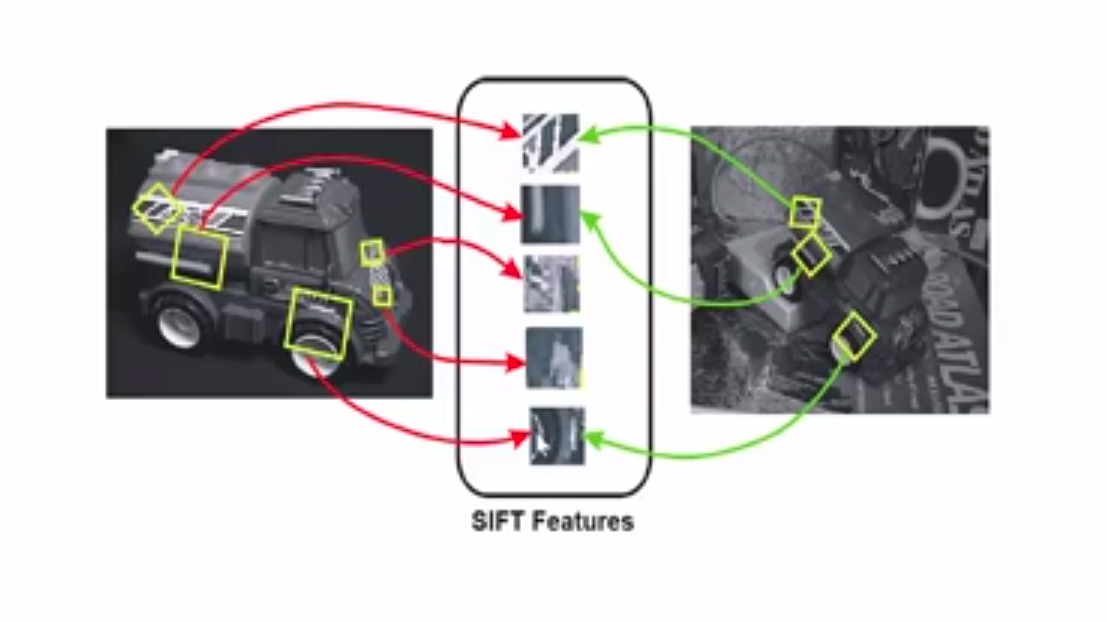
\includegraphics[width=300px,height=125px]{images/sift.png} 
\end{center}

\begin{tcolorbox}[colback=orange!5!white,colframe=orange!75!black]
Write pseudocode \emph{with matrix/array indices} for these steps.

\emph{Notes:} Do this for just one interest point at one scale; ignore the overall interest point orientation; ignore the Gaussian weighting; ignore all normalization post-processing; ignore image boundaries; ignore sub-pixel interpolation and just pick an arbitrary center within the 16$\times$16 for your feature descriptor.
\end{tcolorbox}

\begin{tcolorbox}[enhanced jigsaw,breakable,pad at break*=1mm,colback=white!5!white,colframe=green!75!black,height fixed for=all]
\begin{python}
# You can assume access to the image, x and y gradients, 
# and their magnitudes/orientations.
image = imread("rara.jpg")
grad_x = filter(image, "sobelX")
grad_y = filter(image, "sobelY")
grad_mag = sqrt(grad_x .^2 + grad_y.^2)
grad_ori = atan2(grad_y, grad_x)

# Takes in a interest point x,y location and returns 
# a feature descriptor
def SIFTdescriptor(x, y)
    descriptor = zeros(128,1)
    
    # TODO: Populate descriptor with the right gradient 
    # magnitudes dependent on the gradient orientations



    
    
    
    
    
    
    ################################################
    # YOU MAY USE THIS ADDITIONAL PAGE

    # WARNING: IF YOU DON'T END UP USING THIS PAGE
    # KEEP THESE COMMENTS TO MAINTAIN PAGE ALIGNMENT
    ################################################

    return descriptor
\end{python}
%%%%%%%%%%%%%%%%%%%%%%%%%%%%%%%%% 
% DO NOT REMOVE THIS LINE. IT'S TO MAKE SURE PAGE ALIGNMENT IS CORRECT 
\phantom{}
%%%%%%%%%%%%%%%%%%%%%%%%%%%%%%%%% 
\end{tcolorbox}
% \end{enumerate}

%%%%%%%%%%%%%%%%%%%%%%%%%%%%%%%%%%%


%
% NOT REQUIRED
%

% % Please leave the pagebreak
% \pagebreak
% \paragraph{Q4:} Distance metrics for feature matching.

% \begin{enumerate}[(a)]
%     \item Explain the differences between the geometric interpretations of the Euclidean distance and the cosine similarity metrics. What does this tell us about when each should be used?
% \end{enumerate}

% %%%%%%%%%%%%%%%%%%%%%%%%%%%%%%%%%%%
% \paragraph{A4 (a):} Your answer here.




% %%%%%%%%%%%%%%%%%%%%%%%%%%%%%%%%%%%

% \pagebreak
% \begin{enumerate}[resume*]
%     \item Given a distance metric, what is a good method for feature descriptor matching and why?
% \end{enumerate}

% %%%%%%%%%%%%%%%%%%%%%%%%%%%%%%%%%%%
% \paragraph{A4 (b):} Your answer here.




%%%%%%%%%%%%%%%%%%%%%%%%%%%%%%%%%%%

%
% NOT REQUIRED
%

% \pagebreak
% \paragraph{Secret `something to think about' (ungraded):} 
% In designing a feature point matching algorithm, what characteristics might we wish it to have? How might two world points change in appearance across photographs? Consider that we might allow brightness or contrast changes, or texture changes, or lighting changes, or geometric changes in appearance like rotation and translation in three dimensions or camera perspective effects. All exist between some two photographs of real-world points. 

% We are faced with a fundamental trade-off between feature point invariance (how much variation in appearance I allow and still say that two points are the same) and discriminative power (our ability to say that two points are different or the same at all). 

% How should we design for this trade-off?


\pagebreak
\section*{Discussion Attendance:}
\paragraph{Extra Credit:} \textbf{[2 points]}

Please mark this box only if you've attended the discussion session in person.

\begin{tabular}[h]{ll}
$\square$ & I attended the discussion session on DATE \\
\end{tabular}

\pagebreak
\section*{Feedback? (Optional)}
Please help us make the course better. If you have any feedback for this assignment, we'd love to hear it!


% \pagebreak
% \section*{Any additional pages would go here.}



\end{document}
